
\documentclass[12pt,letterpaper]{article}
\usepackage[utf8]{inputenc}
\usepackage[spanish]{babel}
\usepackage{graphicx}
\usepackage[hidelinks]{hyperref}
\usepackage{hyperref}
\usepackage[left=2cm,right=2cm,top=2.5cm,bottom=2cm]{geometry}
\usepackage{graphicx} % figuras
\usepackage{float} % para usar [H]
\usepackage{amsmath}
\usepackage{stackrel} 
\usepackage{multicol}
\usepackage{multirow}
\usepackage{fancyhdr}
\usepackage[usenames,dvipsnames,svgnames,table]{xcolor}
\usepackage[document]{ragged2e}
\usepackage{enumerate} % enumerados
\renewcommand{\labelitemi}{$-$}
\renewcommand{\labelitemii}{$\cdot$}

\begin{document}
	\begin{titlepage}
		\begin{center}
			\begin{figure}[htb]
				\begin{center}
					
\includegraphics[width=3.5cm]{./img/upt}
				\end{center}
			\end{figure}
			\vspace*{0.15in}
			\begin{Large}
				\textbf{UNIVERSIDAD PRIVADA DE TACNA}\\
			\end{Large}
			\vspace*{0.15in}
			\begin{Large}
				\textbf{FACULTAD DE INGENIERIA} \\
			\end{Large}
			\vspace*{0.1in}
			\begin{Large}
				\textbf{Escuela Profesional de Ingeniería de Sistemas} \\
			\end{Large}
			\vspace*{0.3in}
			\begin{Large}
				\textbf{Actividad/Laboratorio N°04}\\
				\textbf{“Almacenar y consultar una bd grafo con CosmosDB”}\\
			\end{Large}
			\vspace*{0.2in}
			\begin{Large}
				\textbf{CURSO:} \\
			\end{Large}
			\vspace*{0.1in}
			\begin{large}
				Base de Datos II\\
			\end{large}
			\vspace*{0.2in}
			\begin{Large}
				\textbf{DOCENTE:} \\
			\end{Large}
			\vspace*{0.1in}
			\begin{large}
				Ing. Patrick Jose Cuadros Quiroga\\
			\end{large}
			\vspace*{0.3in}
			\begin{large}
				\textbf{ALUMNO:} \\
				\begin{flushleft}
					Risther Jaime Tarqui Montalico  		\hfill	(2017057469) \\
				\end{flushleft}
			\end{large}
			\vspace*{1.3in}
			\begin{large}
				Tacna - Perú\\
			\end{large}
			\vspace*{0.1in}
			\begin{large}
				2020\\
			\end{large}
		\end{center}
	\end{titlepage}
	\include{Secciones/articulo}
	\newpage
	
	\justify
	
	\begin{LARGE}
		\begin{center}
			\textbf{Almacenar y consultar una bd grafo con CosmosDB} \\
		\end{center}
	\end{LARGE}
	\section{OBJETIVO}
	\begin{itemize}
		\item Se creará una cuenta, una base de datos y un gráfico (contenedor) de la API de Azure Cosmos DB Gremlin mediante Azure Portal. Luego, creará y ejecutará una aplicación de consola con un controlador Gremlin de código abierto.
	\end{itemize}
	
	\section{DESARROLLO}
	\subsection{Fotos de finalizacion de Actividad}

\item	Por motivos de creacion de cuenta de Amazon Comos DB, no se pudo completar con el ejercicio de esta actividad.
\begin{enumerate}
	
	
	\item Fotos de finalizacion
	\begin{center}
		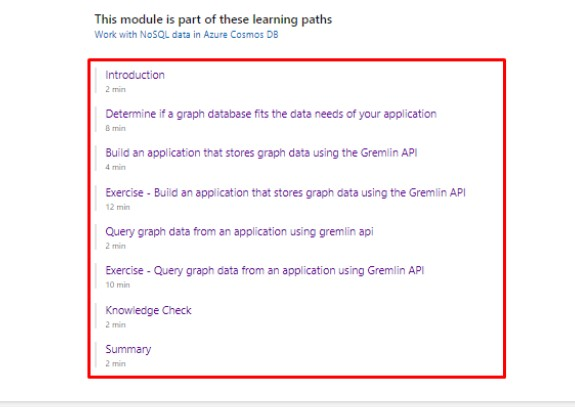
\includegraphics[width=14cm]{./img/f1.jpg} 
	\end{center}
	
	\begin{center}
		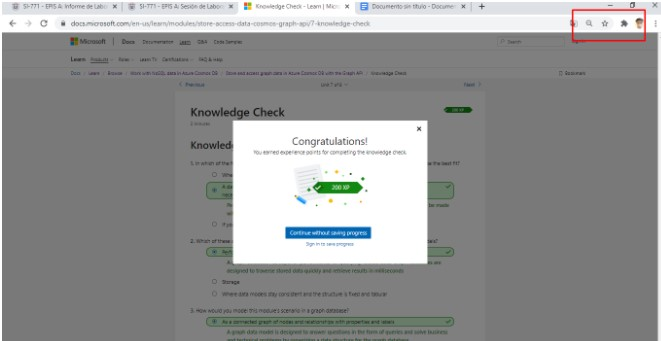
\includegraphics[width=14cm]{./img/f2.jpg} 
	\end{center}
	\begin{center}
		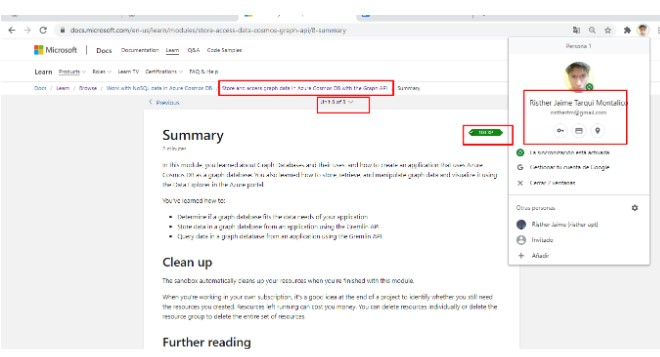
\includegraphics[width=14cm]{./img/f3.jpg} 
	\end{center}
	\begin{center}
		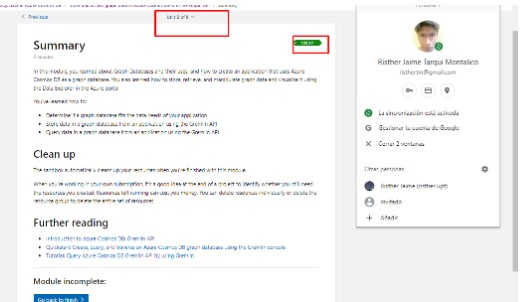
\includegraphics[width=14cm]{./img/f4.jpg} 
	\end{center}
	
	
\end{enumerate}
	
	\subsection{Cree una cuenta de Azure Cosmos DB}
	
\item	Empiece por crear la base de datos en Azure Portal, agregando una cuenta de Azure Cosmos DB que usa la API Graph.
	\begin{enumerate}
		
		\item En el menú de Azure Portal, seleccione Crear un recurso .
		\begin{center}
			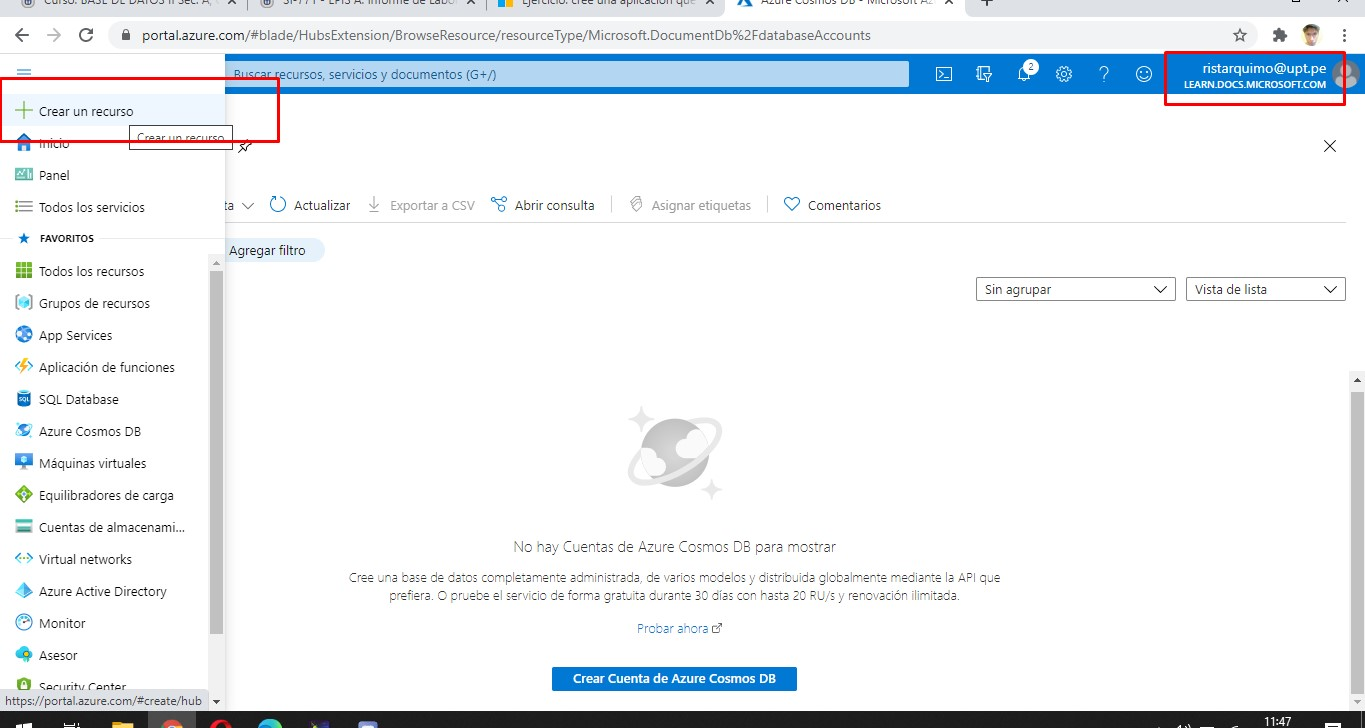
\includegraphics[width=14cm]{./img/1.1.jpg} 
		\end{center}
	
		\item Seleccione Bases de datos > Azure Cosmos DB
		
		\item En el asistente Crear cuenta de Azure Cosmos DB , complete la página Conceptos básicos con estos valores y luego haga clic en Revisar + crear .
		
		\begin{center}
			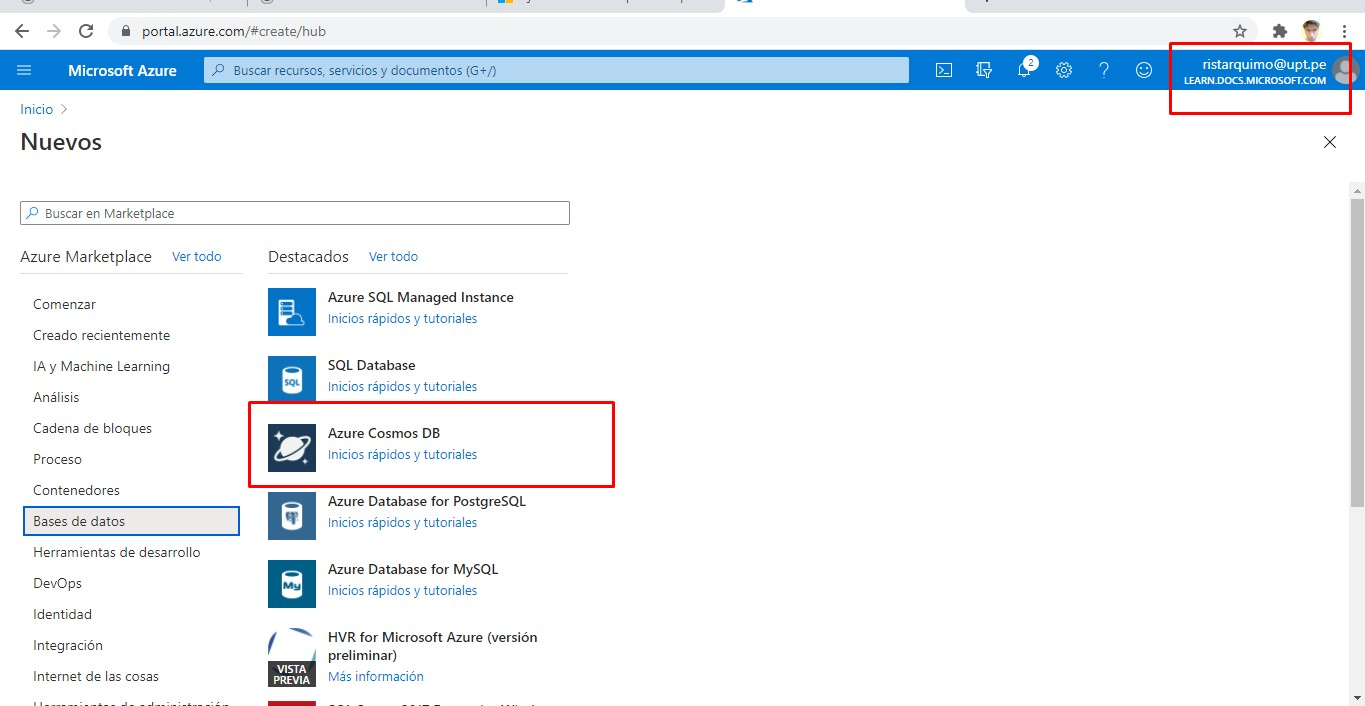
\includegraphics[width=14cm]{./img/1.2.jpg} 
		\end{center}
		
		\itemSeleccione Revisar + Crear , luego Crear .

	
	    
	    
\subsection{Agregar un gráfico }
		
	\begin{enumerate}
		
		\item En el portal de Azure , busque y seleccione la base de datos de Cosmos que creó.
	\\	
		\item En la pestaña Descripción general , copie el valor de Gremlin Endpoint ; utilizará este valor cuando cree su aplicación en la siguiente sección.

		\item Seleccione Explorador de datos y luego seleccione Nuevo gráfico .
		
		\item En el panel Agregar gráfico , ingrese la configuración de su nuevo gráfico. Tome nota de los valores que elija para el ID de la base de datos y el ID del gráfico . Utilizará estos valores cuando cree su aplicación en la siguiente sección.
		\begin{center}
			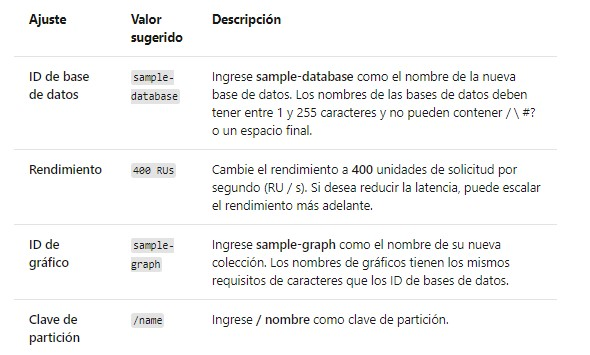
\includegraphics[width=14cm]{./img/2.4.jpg} 
		\end{center}
		\item Seleccione Aceptar para agregar el gráfico a su base de datos.
		
		\item En el panel de navegación izquierdo, en Configuración , seleccione Teclas y luego copie el valor de la CLAVE PRIMARIA . Utilizará este valor cuando cree su aplicación en la siguiente sección.
		
		
	
	
	\subsection{Crear una aplicación .NET Core }


	\begin{enumerate}
		
		\item En Cloud Shell, ingrese los siguientes comandos para crear una nueva aplicación .NET y luego cambie al directorio de su nueva aplicación.
	
		\item Agregue los paquetes necesarios a su aplicación para Gremlin.net y Microsoft.Extensions.Configuration.

	
		\item
		Cree un archivo para la configuración de su aplicación. 
	
		\item Abra su aplicación en el editor de código en línea.
		
		\item Abra su archivo appsettings.json en el editor y agregue la siguiente sintaxis.
		
		\item Para guardar sus cambios, presione Ctrl-S para guardar el archivo.
		
		\item Abra su archivo Program.cs en el editor y agregue las siguientes usingdeclaraciones al principio del archivo.
		
		\item Reemplace el Main()método predeterminado con el siguiente código. Este método lee los valores de configuración del archivo appsettings.json, inicializa la conexión a su cuenta de Azure Cosmos DB mediante el controlador Gremlin.NET, envía una consulta de gráfico al servidor y muestra la cantidad de elementos devueltos por la consulta.
		
		\item Agregue un nuevo AzureAsync()método después del Main()método con el siguiente código. Este método ejecutará la consulta y devolverá un conjunto de resultados que el Main()método utilizará para determinar el número de nodos que devolvió la consulta.
		
		\item Para guardar los cambios, presione Ctrl-S para guardar el archivo y luego presione Ctrl-Q para salir del editor.
		
		\end{enumerate}
	
	
\subsection{Ejecute consultas con su aplicación }
	
	
	\begin{enumerate}
		
		\item Desde el Shell de comandos, ejecute el siguiente comando:
		
		\item  Su nueva cuenta de Azure Cosmos DB no debe contener ningún dato, pero solo para asegurarse, ejecute el siguiente comando para eliminar todos los nodos:
		
		\item  Ahora agregará algunos nodos de productos a su base de datos. Para hacerlo, ejecute los siguientes comandos:
		
		\item  Ahora agregue algunos nodos de categoría a su base de datos. Para hacerlo, ejecute los siguientes comandos:
		
		\item  Verifique que todos sus vértices / nodos se hayan agregado a su base de datos. Para hacerlo, ejecute el siguiente comando:
		
		\item  Ahora agregue algunas relaciones de producto a categoría a su base de datos. Para hacerlo, ejecute los siguientes comandos:
		
		\item Verifique que todos sus bordes / relaciones se hayan agregado a su base de datos. Para hacerlo, ejecute el siguiente comando:
		
	\end{enumerate}


\subsection{Examine sus datos en el portal de Azure }


\begin{enumerate}
	
	\item En el Explorador de datos, expanda la base de datos y los nodos del contenedor y luego haga clic en Gráfico .
	
	\item Haga clic en el botón Ejecutar consulta de Gremlin para usar la consulta predeterminada para ver todos los vértices del gráfico.
	
	
	
\end{enumerate}
		
	\section{CONCLUSIONES}
	\begin{itemize}
			\item No se pudo culminar este laboratorio por problemas con la creacin de cuenta de Amazon Cosmos DB
			
			\item Se realizo La actividad del link propuesto.
			
		\end{itemize}
		
		
	\end{document}